
% xetex expected
\documentclass[xetex,professionalfont]{beamer}

% we want math
\usepackage{amsmath}

% fixes and extensions to amsmath
\usepackage{mathtools}

% additional math symbols
\usepackage{amssymb}

% good-looking fractions in text via \sfrac
\usepackage{xfrac}

% fix spaces after custom commands (see below for examples)
\usepackage{xspace}

% minted allows for fancy syntax highlighting (requires python with pygments)
% usage:
%   \begin{minted}{python}
%   codeb
%   \end{minted}
\usepackage{minted}

% better looking tables
% usage:
%   begin with a \toprule, write a single row of column headings,
%   then add \midrule and after the columns of data we finish with \bottomrule
% example:
%   \begin{tabular}{llr} \toprule
%   Animal & Description & Price \midrule
%   cat & foo & 10 \\
%   dog & bar & 20 \\ \bottomrule
%   \end{tabular}
% note that good tables generally neither have vertical rules nor double rules
\usepackage{booktabs}

% system font support (requires xetex or luatex)
\usepackage{fontspec}
\setmonofont[Scale=0.7]{Cousine} % part of ttf-chromeos fonts on Arch

% multi-language quotes for babel
\usepackage{csquotes}

% easy way to include copyright information
\usepackage{copyrightbox}

% better bibliographies
\usepackage[backend=biber,style=authoryear]{biblatex}

% language support (english,ngerman)
\usepackage[english]{babel}

% minted screws up line spacings ...
\usepackage{setspace}
\usepackage{enumitem}

% -----------------------------------------------------------------------------

% specify PDF metadata
\hypersetup{pdftitle={CVSP VO - Specific Object Recognition},pdfsubject={},pdfauthor={Christopher Pramerdorfer}}

% copyright font style
\makeatletter\renewcommand{\CRB@setcopyrightfont}{\tiny\color{lightgray}}

% add bib file
\addbibresource{literature.bib}

% use tuwcvl beamer theme
\usetheme{tuwcvl}

% add some space between lines
\setstretch{1.4}

% but not for minted environments
\AtBeginEnvironment{minted}{\singlespacing}

% fix itemize

\setlist{nolistsep}
\setitemize{itemsep=-1mm,label=\usebeamerfont*{itemize item}%
  \usebeamercolor[fg]{itemize item}
  \usebeamertemplate{itemize item}}

% -----------------------------------------------------------------------------

% common english abbreviations
\newcommand{\ie}{\mbox{i.e.}\xspace} % i.e.
\newcommand{\eg}{\mbox{e.g.}\xspace} % e.g.

% math - argmin and argmax
\DeclareMathOperator*{\argmin}{arg\,min}
\DeclareMathOperator*{\argmax}{arg\,max}

% shortcuts for number ranges
\newcommand{\NN}{\mathbb{N}}
\newcommand{\ZZ}{\mathbb{Z}}
\newcommand{\QQ}{\mathbb{Q}}
\newcommand{\RR}{\mathbb{R}}

% bold vectors
\renewcommand{\vec}[1]{\ensuremath{\mathbf{#1}}}

% vector shortcuts
\newcommand{\va}{\vec{a}}
\newcommand{\vb}{\vec{b}}
\newcommand{\vc}{\vec{c}}
\newcommand{\ve}{\vec{e}}
\newcommand{\vr}{\vec{r}}
\newcommand{\vs}{\vec{s}}
\newcommand{\vt}{\vec{t}}
\newcommand{\vu}{\vec{u}}
\newcommand{\vv}{\vec{v}}
\newcommand{\vw}{\vec{w}}
\newcommand{\vx}{\vec{x}}
\newcommand{\vy}{\vec{y}}
\newcommand{\vz}{\vec{z}}

\newcommand{\bth}{\boldsymbol{\theta}}

% highlight
\newcommand{\highlight}[1]{\textcolor{tuwcvl_inf_red}{\textbf{#1}}}

% make emph red
\let\oldemph\emph
\renewcommand\emph[1]{\textcolor{tuwcvl_inf_red}{#1}}

% -----------------------------------------------------------------------------

\title{Computer Vision Systems Programming VO}
\subtitle{Specific Object Recognition}
\author{Christopher Pramerdorfer}
\institute{Computer Vision Lab, Vienna University of Technology}

\begin{document}

% -----------------------------------------------------------------------------

\begin{frame}
\maketitle
\end{frame}

% -----------------------------------------------------------------------------

\begin{frame}
\frametitle{Topics}

Introduction to object recognition \\
Specific object recognition (rigid, nonrigid)

\bigskip
\begin{center}
    \copyrightbox[b]
    {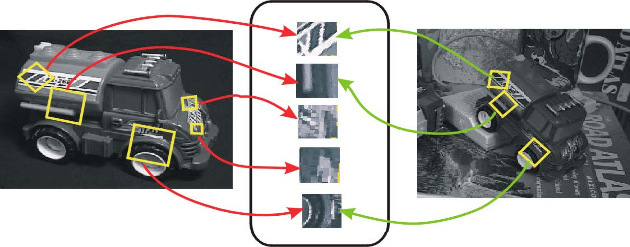
\includegraphics[width=7cm]{figures/local-feature-matching.jpg}}
    {\centering Image from \cite{grauman2011}}
\end{center}

\end{frame}

% -----------------------------------------------------------------------------

\begin{frame}
\frametitle{Object Recognition}

Fundamental problem in Computer Vision

\bigskip
Many applications
\begin{itemize}
	\item Panorama stitching, 3D reconstruction
	\item HCI and surveillance (face recognition)
	\item Image understanding (recall Fei-Fei Li's TED talk)
\end{itemize}

\end{frame}

% -----------------------------------------------------------------------------

\begin{frame}
\frametitle{Object Recognition}
\framesubtitle{Taxonomy -- Instance vs.\ Category}

\emph{Instance recognition} (\emph{specific object recognition})
\begin{itemize}
	\item Recognize a specific, uniquely looking object % even if differences are only in details
	\item Face of a certain person, the Eiffel tower
\end{itemize}

\bigskip
\emph{Object category recognition}
\begin{itemize}
	\item Recognize objects of a certain category % note that categories are hierarchical ... like panda bears - bears - mammals - animals. some test databases reflect this, like ImageNet. obviously, the more general the category, the harder the recognition task
	\item Human faces, buildings
\end{itemize}

\end{frame}

% -----------------------------------------------------------------------------

\begin{frame}
\frametitle{Object Recognition}
\framesubtitle{Taxonomy -- Instance vs.\ Category}

\begin{center}
\begin{tikzpicture}
    \node[anchor=south west,inner sep=0] (image) at (0,0) {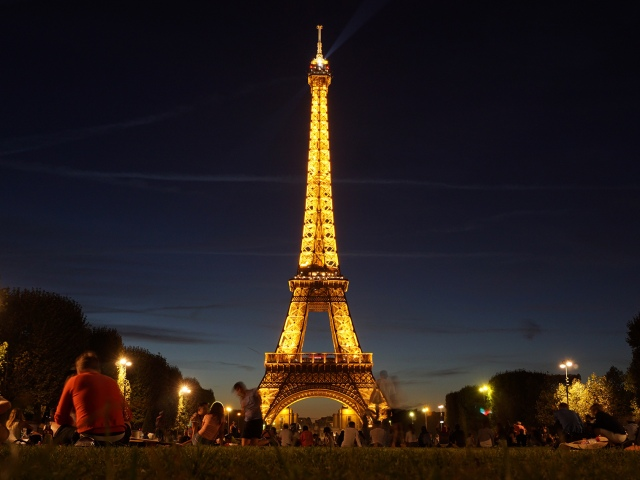
\includegraphics[width=8cm]{figures/eiffel-tower.jpg}};
    \begin{scope}[x={(image.south east)},y={(image.north west)}]
        \node[green] at (0.205,0.94) {category: building};
        \node[green] at (0.24,0.87) {instance: Eiffel tower};
    \end{scope}
\end{tikzpicture}
\end{center}

\end{frame}

% -----------------------------------------------------------------------------

\begin{frame}
\frametitle{Object Recognition}
\framesubtitle{Taxonomy -- Classification vs.\ Detection}

\emph{Object classification}
\begin{itemize}
	\item Recognize main object in image % disregarding the rest / we assume that there is a dominant object in the image (maybe we detected the object and cropped the image in a preprocessing step)
	\item Location and other objects not relevant
\end{itemize}

\bigskip
\emph{Object detection}
\begin{itemize}
	\item Recognize multiple objects, possibly of different category
\end{itemize}

\end{frame}

% -----------------------------------------------------------------------------

\begin{frame}
\frametitle{Object Recognition}
\framesubtitle{Taxonomy -- Classification vs.\ Detection}

\begin{center}
\begin{tikzpicture}
    \node[anchor=south west,inner sep=0] (image) at (0,0) {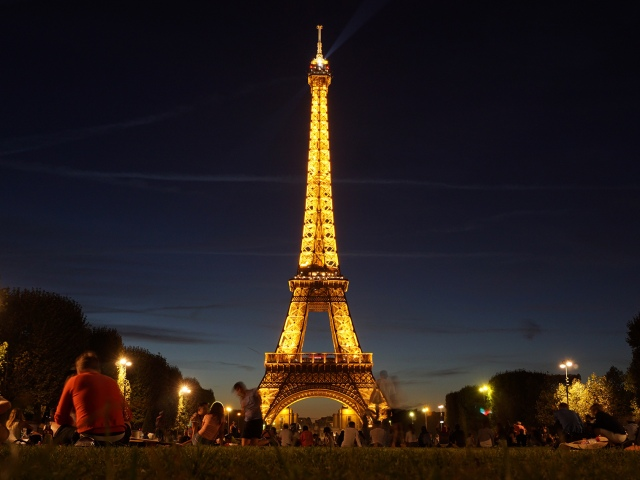
\includegraphics[width=8cm]{figures/eiffel-tower.jpg}};
    \begin{scope}[x={(image.south east)},y={(image.north west)}]
        \draw[red,ultra thick] (0.35,0.08) rectangle (0.65,0.97);
        \node[red] at (0.75,0.54) {building};
        \draw[red,ultra thick] (0.08,0.08) rectangle (0.21,0.28);
        \node[red] at (0.145,0.32) {person};
        \node[green] at (0.1,0.94) {building}; % the class of the image (classification task)
    \end{scope}
\end{tikzpicture}
\end{center}

\end{frame}

% -----------------------------------------------------------------------------

\begin{frame}
\frametitle{Object Recognition}
\framesubtitle{Challenges}

Instances of same category can look very differently
\begin{itemize}
    \item Illumination, pose, viewpoint, occlusions, background
\end{itemize}

\medskip
\begin{center}
    \copyrightbox[b]
    {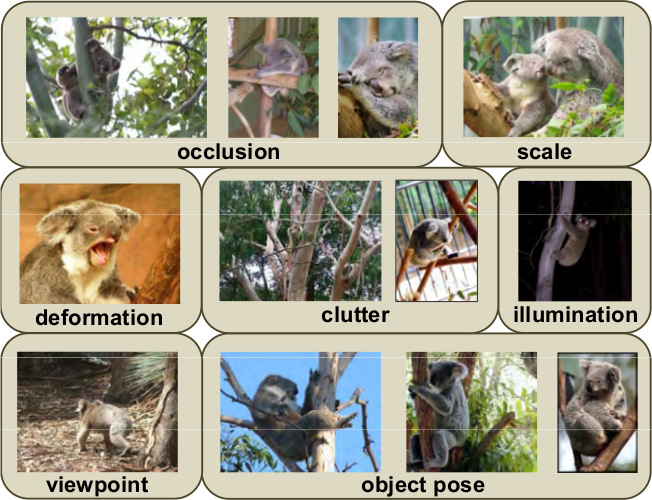
\includegraphics[width=6cm]{figures/challenges.jpg}}
    {\centering Image from \cite{grauman2011}}
\end{center}

\end{frame}

% -----------------------------------------------------------------------------

{
\setbeamertemplate{footline}{}
\begin{frame}

\begin{tikzpicture}[remember picture,overlay]
\fill[white] (current page.north west) rectangle (current page.south east);
\end{tikzpicture}

\end{frame}
}

% -----------------------------------------------------------------------------

\begin{frame}
\frametitle{Specific Planar Object Detection}

We want to detect specific planar objects (e.g. markers, books)
\begin{itemize}
	\item Comparatively easy problem
\end{itemize}

\bigskip
Challenges
\begin{itemize}
	\item Unknown object pose and scale
	\item Partial occlusions
	\item Illumination
\end{itemize}

\end{frame}

% -----------------------------------------------------------------------------

\begin{frame}
\frametitle{Specific Planar Object Detection}

\begin{center}
    \copyrightbox[b]
    {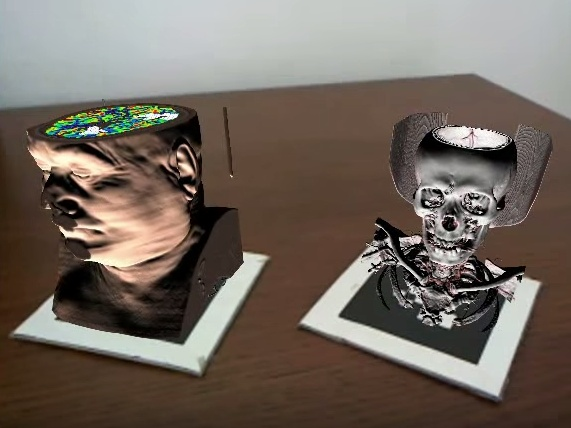
\includegraphics[width=7cm]{figures/marker-ar.jpg}}
    {\centering Image from \href{https://www.youtube.com/watch?v=ChGW2Jogdjs}{\texttt{youtube.com}}}
\end{center}

\end{frame}

% -----------------------------------------------------------------------------

\begin{frame}
\frametitle{Specific Planar Object Detection}
\framesubtitle{Selecting $\vx$ and $\vw$}

Our problem formulation is  % this is what is used normally because it is very flexible
\begin{itemize}
	\item Given a pixel location in a query image
	\item Predict location in reference image of sought object  % will be out of bounds inf the original pixel location does not lie on the object
\end{itemize}

\bigskip
So we know how to select $\vx$ and $\vw$
\begin{itemize}
	\item $\vx=(x,y)$ : location in query image
	\item $\vw=(u,v)$ : corresponding location in reference image
\end{itemize}

\end{frame}

% -----------------------------------------------------------------------------

\begin{frame}
\frametitle{Specific Planar Object Detection}
\framesubtitle{Selecting $\vx$ and $\vw$}

\begin{center}
    \copyrightbox[b]
    {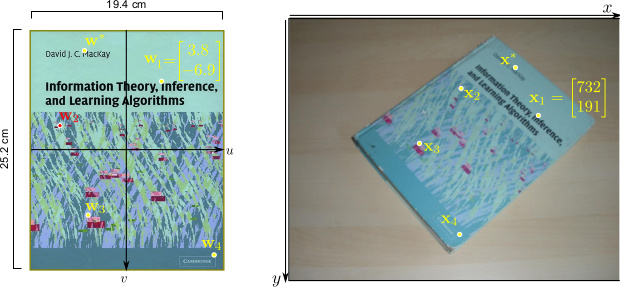
\includegraphics[width=10cm]{figures/book-xw.jpg}}
    {\centering Image from \cite{prince12}}
\end{center}

\end{frame}

% -----------------------------------------------------------------------------

\begin{frame}
\frametitle{Specific Planar Object Detection}
\framesubtitle{Model Selection}

Images of planar objects are always related by a \emph{homography} $\boldsymbol{\Phi}$
\begin{itemize}
	\item $3\times3$ matrix mapping between corresponding points
\end{itemize}

\bigskip
In homogeneous coordinates this means that
\[
	\lambda
	\begin{pmatrix}
		u \\ v \\ 1
	\end{pmatrix}
	= \boldsymbol{\Phi}
	\begin{pmatrix}
		x \\ y \\ 1
	\end{pmatrix}
\]

\end{frame}

% -----------------------------------------------------------------------------

\begin{frame}
\frametitle{Specific Planar Object Detection}
\framesubtitle{Model Selection}

The model of choice is thus (disregarding noise)
\[
	\vw=\Gamma(\vx)=
	\begin{pmatrix}
		u \\ v
	\end{pmatrix}\quad,\quad
	\lambda
	\begin{pmatrix}
		u \\ v \\ 1
	\end{pmatrix}
	= \boldsymbol{\Phi}
	\begin{pmatrix}
		x \\ y \\ 1
	\end{pmatrix}
\]

\end{frame}

% -----------------------------------------------------------------------------

\begin{frame}
\frametitle{Specific Planar Object Detection}
\framesubtitle{Learning Model Parameters}

We again learn parameters $\bth$ from samples $\{\vx_i,\vw_i\}_{i=1}^n$
\begin{itemize}
	\item $\bth$ contains 9 parameters comprising $\boldsymbol{\Phi}$
\end{itemize}

\bigskip
Usually no exact solution because of noisy $\vx_i$
\begin{itemize}
	\item Formulate as a \emph{least squares problem} instead
\end{itemize}

\[
	\hat{\bth}=\argmin_{\bth} \left[\sum_{i=1}^n (\vw_i-\Gamma(\vx_i))^\top(\vw_i-\Gamma(\vx_i)) \right]
\]

\end{frame}

% -----------------------------------------------------------------------------

\begin{frame}
\frametitle{Specific Planar Object Detection}
\framesubtitle{Learning Model Parameters}

This least squares approach is optimal
\begin{itemize}
	\item If noise is distributed normally with spherical covariance % with spherical covariance (same, independent noise affecting x1 and x2)
\end{itemize}

\bigskip
This is a nonlinear optimization problem
\begin{itemize}
	\item Solvable using any general nonlinear least squares solver % depends on a good initial estimate of the parameters (because there is no global optimum)
	\item OpenCV has an own function \texttt{findHomography}
\end{itemize}

\end{frame}

% -----------------------------------------------------------------------------

\begin{frame}
\frametitle{Specific Planar Object Detection}

But how can we compute $\{\vx_i,\vw_i\}_{i=1}^n$ automatically?
\begin{itemize}
	\item Next lecture
\end{itemize}

\end{frame}

% -----------------------------------------------------------------------------

\setstretch{1}
\renewcommand\emph[1]{\oldemph{#1}}

\begin{frame}
\frametitle{Bibliography}

\printbibliography

\end{frame}

\end{document}
